\documentclass[a4paper,11pt]{article}
\usepackage{booktabs} % Provides professional-quality horizontal rules
\usepackage{float} % Required for [H] placement
\usepackage{tikz}
\usepackage{hyperref}
\usepackage{graphicx} 
% \graphicspath{ {./images/} } % Optional: Specifies the folder where your images are saved
% \usepackage[bottom=1.5in]{geometry} // push page footer down 
\setlength{\footskip}{100pt}
\usepackage[skip=4pt, font=tiny]{caption} 

\hypersetup{
    colorlinks=true,    % True removes the default red/green border boxes
    linkcolor=blue,     % Colors internal links (like the TOC) blue
    urlcolor=cyan       % Colors external URLs cyan
}

\newcommand{\newpagex}{
    \newpage
    \vspace*{-7\baselineskip} % Pulls text up by one line
}

\author{Hectron} 

\title{Getting Started NBA App}

\begin{document}
    \maketitle
    \tableofcontents
    \newpagex
    \noindent

    \section{Description}
        Document informs the user how to start the application residing in the nba\_app  directory of repository ReactApps. 
        Applications were developed on MacOS \(Sonoma\). The following programming languages were used throughout fullstack development.
        \begin{itemize}
            \item \textbf{FrontEnd:} \newline \textmd{Typescript - imperative}
            \item \textbf{Backend}: \newline  \textmd{Postgres - declarative}
            \item \textbf{Script}: \newline  \textmd{Bash - imperative}
        \end{itemize}

    \section{Run Application}
        \begin{itemize}
            \item  Open Docker. If Docker is not installed, please download at \hypersetup{colorlinks=false,urlcolor=black } \url{https://www.docker.com/products/docker-desktop/} 
            \item Start/Configure Postgres Database (Docker Container Instance) 
            \begin{itemize}
                \item Change directory to nba\_app/database
                \item run run.sh 
            \end{itemize}
            \item Start Monitor Service.
                \newline 
            The highest priority service. All request are handled by the monitor service. The start monitor must be running for proper operation of the application. 
                \begin{itemize}
                \item Change directory to nba\_app
                \item run server/main.sh \quad \small \textit{Monitor service is now running }
            \end{itemize}

            \item Open web browser; request application at address and port \url{ http://127.0.0.1:50214/ }
        \end{itemize}
            

    \section{Figures}

        \noindent
        % O(nlog\_{2}(n)) search .This is a\_test. 
        \vspace*{-2\baselineskip} % Pulls text up by one line
        
        \begin{figure}[H]
            
            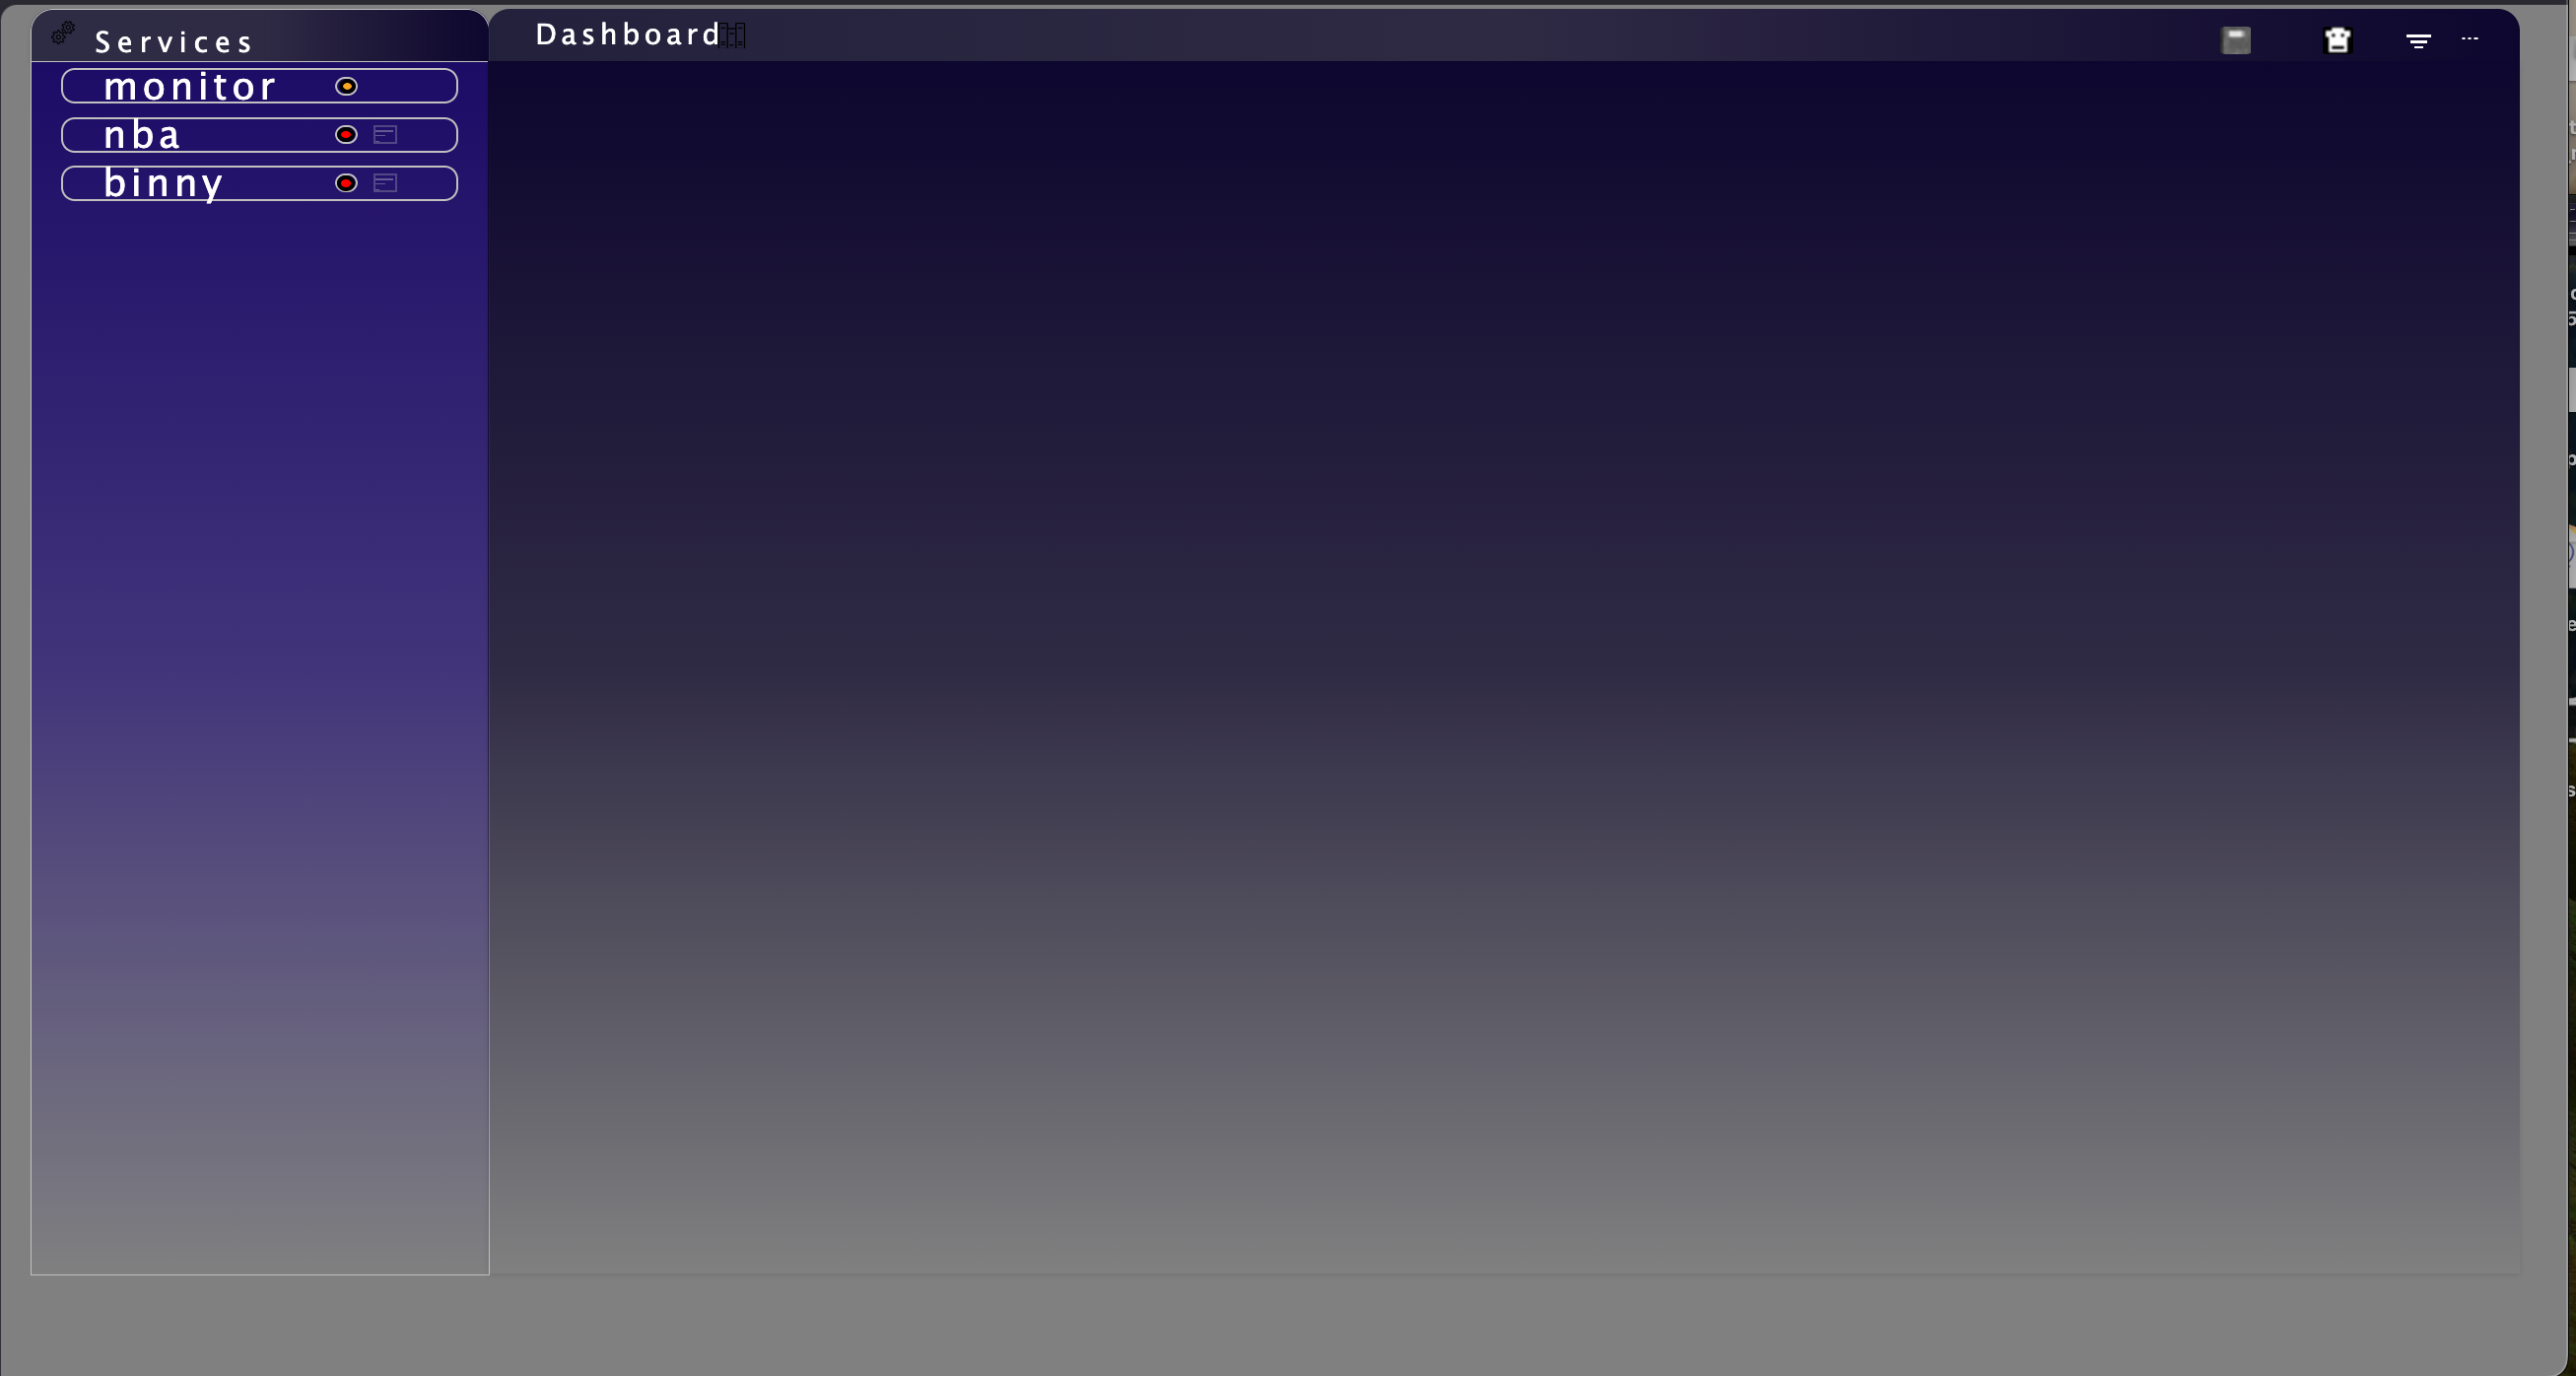
\includegraphics[width=1.0\textwidth, height=0.27\textheight]{image0}
            
            \caption{Home Page}
        
            \label{fig:home}

        \end{figure}
    
         \newpagex

        \begin{figure}[H]
            
            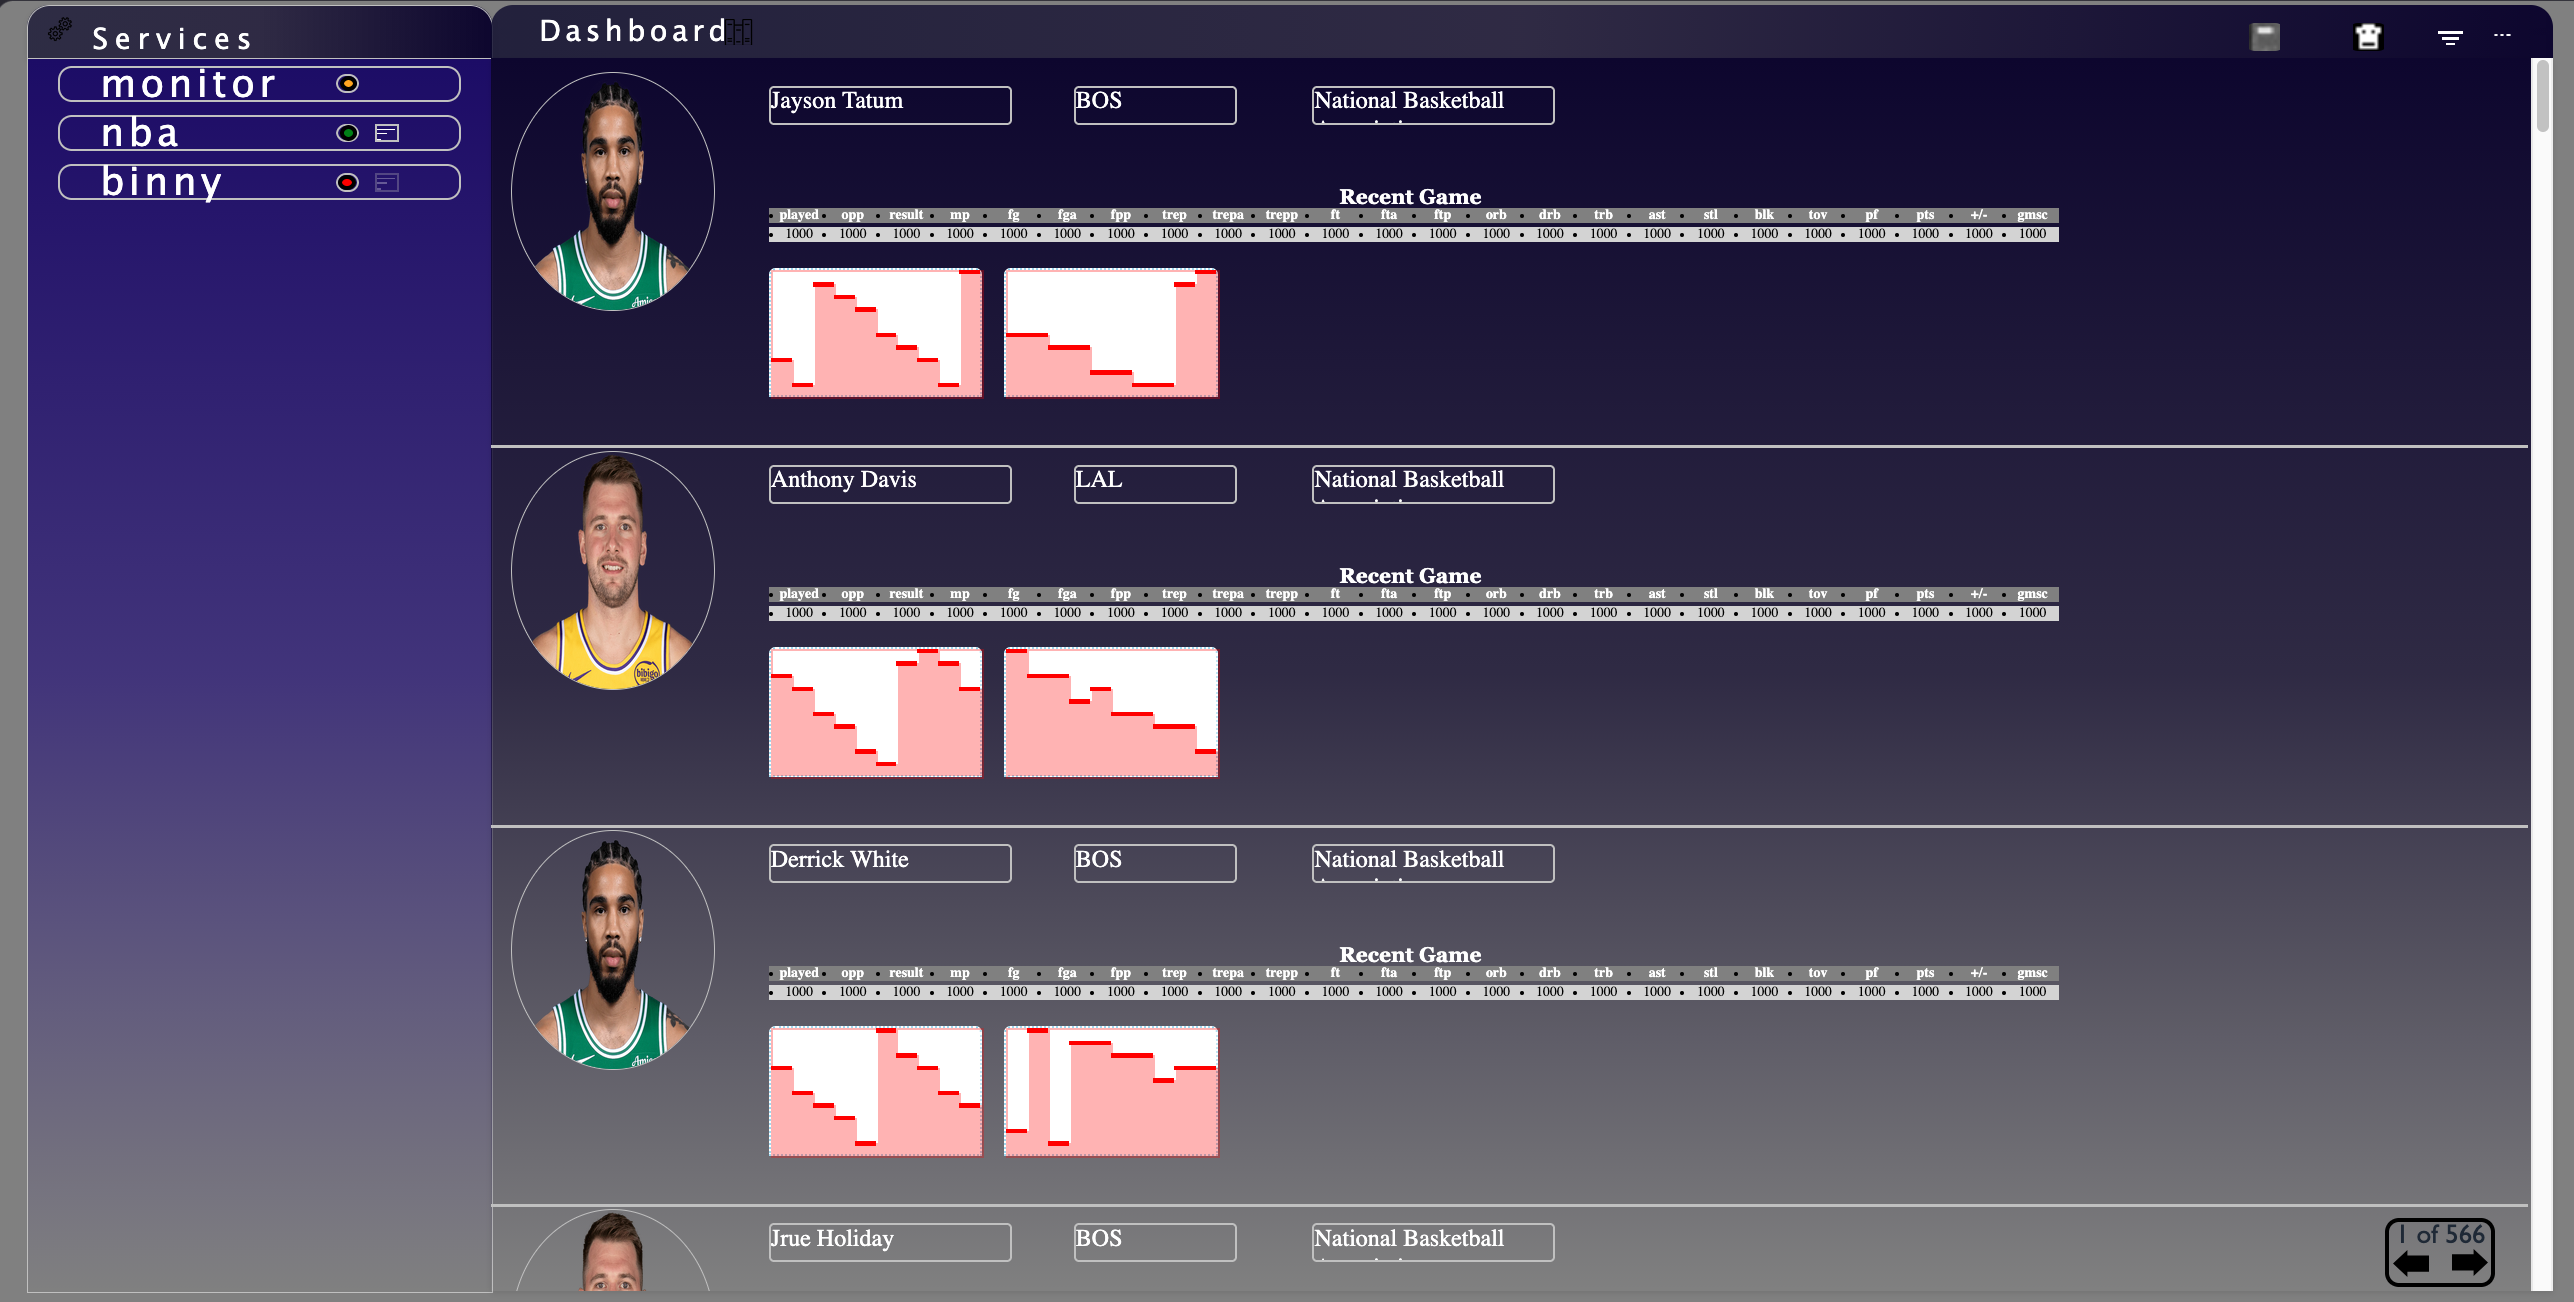
\includegraphics[width=1.0\textwidth, height=0.27\textheight]{image1}
            
            \caption{\textbf{GET} NBA Service}
        
            \label{fig:nba}

        \end{figure}

\end{document}